\documentclass{article}
\setlength{\parindent}{0ex}
\setlength{\parskip}{2ex}
\usepackage{graphicx, amssymb, url}

\begin{document}

\author{Igor Serebryany}
\title{The EWE Webserver \\ CMSC 23300}
\maketitle
\clearpage

\section{Overview}

The EWE (Igor WEbserver) webserver is a fully-functional HTTP server written in Python.
Its is ideally suited for evaluating the relative performance of different threading models, but it can also be used as a webserver for small servers.
With its object-oriented design, it is designed from the ground up to be modular and easily extensible.
EWE is a great example of the Python coding idioms, and thus can also be useful as a Python reference codebase.

This document describes in detail the features and operation of EWE, gives an overview of its performance and lists known bugs in the code.
Please feel free to contact the author of EWE, Igor Serebryany, at \texttt{igor47@monksofcool.org} with any questions, comments or bug reports.
You may also get the most recent revision of EWE at \url{http://igor.monksofcool.org/projects/webserver}.
This URL is accessible a web browser for the latest version, and can also be used as an SVN read-only repository to get a recent version and to see previous versions.

\section{Operation}
\subsection{System requirements}
EWE was designed on a Gentoo GNU/Linux platform running Python 2.4.
It as also been tested on Debian with Python 2.3.
The code tries to be portable as much as possible, and should work with any relatively recent version of Python.
EWE has not been tested under Windows, and would probably not work there without some modification because it utilizes some UNIX-only system calls.

\subsection{Files}
EWE is defined in 5 Python files - \texttt{ewe.py, baseProcessor.py, processors.py, logger.py} and \texttt{features.py}.
\begin{description}
\item[ewe.py] This is the main server file.
When run, it will first parse all the configuration options and start the logger and request processor.
It will then listen for incoming connections and pass the resulting connections off to the processor.
\item[logger.py] This is the logger definition.
The code in this file will open the logfile and send incoming log messages to it or to the screen, depending on the log level.
\item[processors.py] This file contains the definitions for the different concurrency models.
The objects in this file wrap baseProcessor.py and interact with it to process requests.
\item[baseProcessor.py] This file contains the processor object which does all of the request handling.
The object has methods to read data from a connection, parse it, create the response and send it off.
\item[features.py] This file contains the definitions for various supporting features of the baseProcessor, including CGI support and the directory-index generating function.
\end{description}

\subsection{Command-line operation}
EWE is operated from the commandline by running the main Python script, \texttt{ewe.py}.
It accepts two optional command-line arguments:

\parbox{3in}{\centering ewe.py [-f|-t|-p] [port]}

\begin{tabular}{|l|l|}
\hline
Option & Effect \\
\hline
-f & Fork a new process for each request \\
-t & Start a new thread for each request \\
-p & Create a pool of worker threads and serve\\
   & new requests from the available pool \\
\hline
port & Listen for new connections on the given port \\
\hline
\end{tabular}

\subsection{Configuration}\label{config}
\begin{table}[h]
\begin{tabular}{|l|c|l|}
\hline
Option & Default Value & Description \\
\hline
concurrency & "none" & The default concurrency model (overriden by commandline) \\
port & 4000 & The default port number (overridden by commandline) \\
poolthreads & 5 & Number of worker threads to create if using -p \\
indexes & True & Should EWE generate directory indexes? \\
persistent & True & Should EWE use persistent connections? \\
loglevel & 0 & Log all messages below this level \\
logfile & ewe.log & Log messages are written to this file \\
defaultindex & "index.html" & The default file to open in a directory request\\
documentroot & "htdocs" & The physical path to \url{/} URLs \\
cgipath & "cgi-bin" & The physical path to \url{/cgi-bin} URLs \\
\hline
\end{tabular}
\caption{EWE Configuration Parameters}\label{config}
\end{table}

EWE accepts further configuration parameters, outlined in \ref{config}.
These parameters are stored in a Python dictionary in ewe.py and can be changed by editing the file.

\section{Code Features}
\subsection{Directory Indexes}
When an HTTP request URL refers to a directory instead of a file, EWE will generate an index of the directory as the response.
This feature can be deactivated by the `indexes' option (see section \ref{config}).

\subsection{Persistence}
EWE supports persistent connections.
With this feature enabled, EWE can reuse a single TCP connection with a client for several transactions.
The feature can be enabled and disabled as per section \ref{config}.

\subsection{CGI}\label{cgi}
EWE supports basic CGI operations.
For requests with URLs beginning with \url{/cgi-bin/}, EWE will look in the location given by the "cgipath" configuration option for the file requested.
If the file is found and EWE has execute privileges on it, the file will be executed and its output sent as the response to the HTTP request.

If the required conditions to run the file are not met, normal parsing takes place.
This means that if the cgipath directive points into the document root, the requested file may simply be served as a regular document.

EWE supports the POST method for CGI documents.
The CGI executor will pass the request entity to the CGI script as its standard input.
The server will return a 405 error if the POST method is requested for documents other then CGI scripts.
If this happens and persistent connections are enabled, EWE will also close the persistent connection since it is unable to deal with the POST input outside the CGI context.

\section{Performance Comparison}
\subsection{General comparison}
The statistics in table \ref{perfChart} were collected utilizing httperf with the parameters given in the project description.
For this experiment, Apache ran on \url{s8.diperf.cs.uchicago.edu} and EWE ran on \url{west-coast-champion.cs.uchicago.edu}, a dual-processor P4-3Ghz machine.
HTTPerf ran from \url{trail-blazer.cs.uchicago.edu}, a P4-2.8GHz machine.
Where errors a present, the type of error is reported after the number of errors of that type.
\begin{description}
\item[ct] Client timeout
\item [st] Socket timeout
\item [ref] Connection refused
\item [res] Connection reset
\end{description}

\begin{table}[h]
\begin{tabular}{|l|c|c|c|c|c|}
\hline
Statistic & Apache & EWE basic & EWE -f & EWE -t & EWE -p \\
\hline
Connections & 1000 & 1000 & 1000 & 1000 & 1000 \\
Requests & 10000 & 1145 & 10000 & 9784 & 2270 \\
Replies & 100000 & 1140 & 10000 & 9760 & 2270 \\
Duration (s)& 9.873 & 251.709 & 46.421 & 59.8 & 189.9 \\
Connection Rate (conn/s)& 101.3 & 4 & 21.5 & 16.7 & 5.3 \\
Request Rate (req/s)& 1012.8 & 4.5 & 215.4 & 163.5 & 11.9 \\
Avg. Reply Rate (req/p)& 1663.8 & 4.6 &218.5 & 177.5 & 11.9 \\
Reply Time (ms)& 68.7 & 2142.9 & 82.4 & 933.7 & 101.1 \\
Net I/O (KB/s)& 426.3 & 1.4 & 65.4 & 49.6 & 3.6 \\
Errors & 0 & 881(st) 5(res) & 0 & 24(res)& 773 (ct) \\
\hline
\end{tabular}
\caption{Performance Comparison - 64byte}\label{perf64}
\end{table}

\begin{table}[h]
\begin{tabular}{|l|c|c|c|c|c|}
\hline
Statistic & Apache & EWE basic & EWE -f & EWE -t & EWE -p \\
\hline
Connections & 1000& 1000 & 1000 & 1000 & 1000\\
Requests & 10000& 1232 & 10000 & 9163 & 2410\\
Replies & 10000& 1230 & 10000 & 9070 & 2410\\
Duration (s)& 10.260& 218.798 & 46.494 & 73.041 & 189.987\\
Connection Rate (conn/s)& 97.5& 4.6 & 21.5 & 13.7 & 5.3\\
Request Rate (req/s)& 974.7 & 5.6 & 215.1 & 125.4 & 12.7\\
Avg. Reply Rate (req/p)& 927.1 & 5.7 & 219.3 & 129.1 & 13.0\\
Reply Time (ms)& 58.7 & 979.2 & 96.0 & 1071.5 & 110.1\\
Net I/O (KB/s)& 1310.7 & 5.9 & 263.8 & 152.4 & 15.6\\
Errors & 0 & 875(st) & 0 & 93(res) & 759(st)\\
\hline
\end{tabular}
\caption{Performance Comparison - 1024byte}\label{perf1024}
\end{table}

\begin{table}[h]
\begin{tabular}{|l|c|c|c|c|c|}
\hline
Statistic & Apache & EWE basic & EWE -f & EWE -t & EWE -p \\
\hline 
Connections & 1000 & 1000 & 1000 & 1000 & 1000  \\
Requests & 5000 & 3609 & 5000 & 5000 & 4988 \\
Replies & 5000 & 3385 & 5000 & 5000 & 4985 \\
Duration (s)& 11.062 & 246.5 & 22.211 & 34.387 & 59.706 \\
Connection Rate (conn/s)& 90.4 & 4.1 & 45 & 29.1 & 16.7 \\
Request Rate (req/s)& 452 & 14.6 & 224.1 & 145.3 & 83.5 \\
Avg. Reply Rate (req/p)& 429.0 & 13.8  & 246.8 & 166.3 & 88.5 \\
Reply Time (ms)& 210.5 & 2298.4 & 280.6 & 836.6 & 906.6 \\
Net I/O (KB/s)& 7270.5 & 219.0 & 3588.6 & 2317.3 & 1331 \\
Errors & 0  & 99 (st) 224(cr) & 0 & 0 & 3 (res) \\
\hline
\end{tabular}
\caption{Performance Comparison - 16K}\label{perf16K}
\end{table}

\begin{table}[h]
\begin{tabular}{|l|c|c|c|c|c|}
\hline
Statistic & Apache & EWE basic & EWE -f & EWE -t & EWE -p \\
\hline 
Connections & 1000 & 1000 & 1000 & 1000 & 1000 \\
Requests & 2904 & 1263 & 2858 & 2866 & 1701 \\
Replies & 2856 & 1092 & 2787 & 2799 & 1701 \\
Duration (s)& 46.819 & 247 & 46.03 & 46.32 & 189.9 \\
Connection Rate (conn/s)& 21.4 & 4 & 21.7 & 21.6 & 5.3 \\
Request Rate (req/s)& 62.0 & 5.1 & 62.1 & 61.9 & 9.0 \\
Avg. Reply Rate (req/p)& 61.1 & 4.5 & 61.8 & 61.5 & 9.0 \\
Reply Time (ms)& 2049.1 & 5852.6 & 1303.2 & 1011.5 & 426.2 \\
Net I/O (KB/s)& 7680.8 & 556.1 & 7615.9 & 7601 & 1126.2 \\
Errors & 48(cr) & 465(st) 171(res) & 71(res) & 67 & 433(st) \\
\hline
\end{tabular}
\caption{Performance Comparison - 128K}\label{perf128K}
\end{table}

A number of conclusions can be made from tables \ref{pref64} to \ref{pref128K}.
The non-concurrent model of EWE has the worst performance, but the pool of threads model is a close second.
Both of these models perform poorly for the same reason | a large number of socket timeout errors.
These models are both limited in the number of clients they can serve - the basic model, a single client, and the pool of threads model only as many clients as there are threads in the pool.
Thus, many requests will timeout, and the requests that do succeed must wait until a previous client is finished using the server.

An interesting peculiarity of EWE is that the forked concurrency model performs better then the threaded model.
Traditional systems wisdom dictates that it takes much longer to fork a new process then to create a new thread.
In the case of EWE, however, each new thread created must instantiate a baseProcessor object while each new thread gets an existing copy of one.
This fact actually causes a reversal, with forked processors experiencing the fewest errors and rivaling Apache's performance.

In addition, EWE is limited in the number of threads it can create, since a process is limited in the number of file descriptors it is allowed to have.
Thus, while EWE can fork processes almost indefinitely, it must stop generating new threads beyond a certain limit and wait until some existing ones have terminated.
This is the reason that the threaded model behaves much better when there are fewer requests, as in table \ref{pref128K}.

\subsection{Optimal Performance}
In order to find the performance peak of each server model, httperf was driven with a distributed autobench session which utilized four machines as clients: \texttt{gotham.cs.uchicago.edu, silver-star.cs.uchicago.edu, barnacle-bill.cs.uchicago.edu} and \texttt{admiral.cs.uchicago.edu}.
Figures \ref{perfpeak1} and \ref{perfpeak2} demonstrate the performance of EWE as well as Apache as s8 at various request rates.
\begin{figure}[ht]\centering
        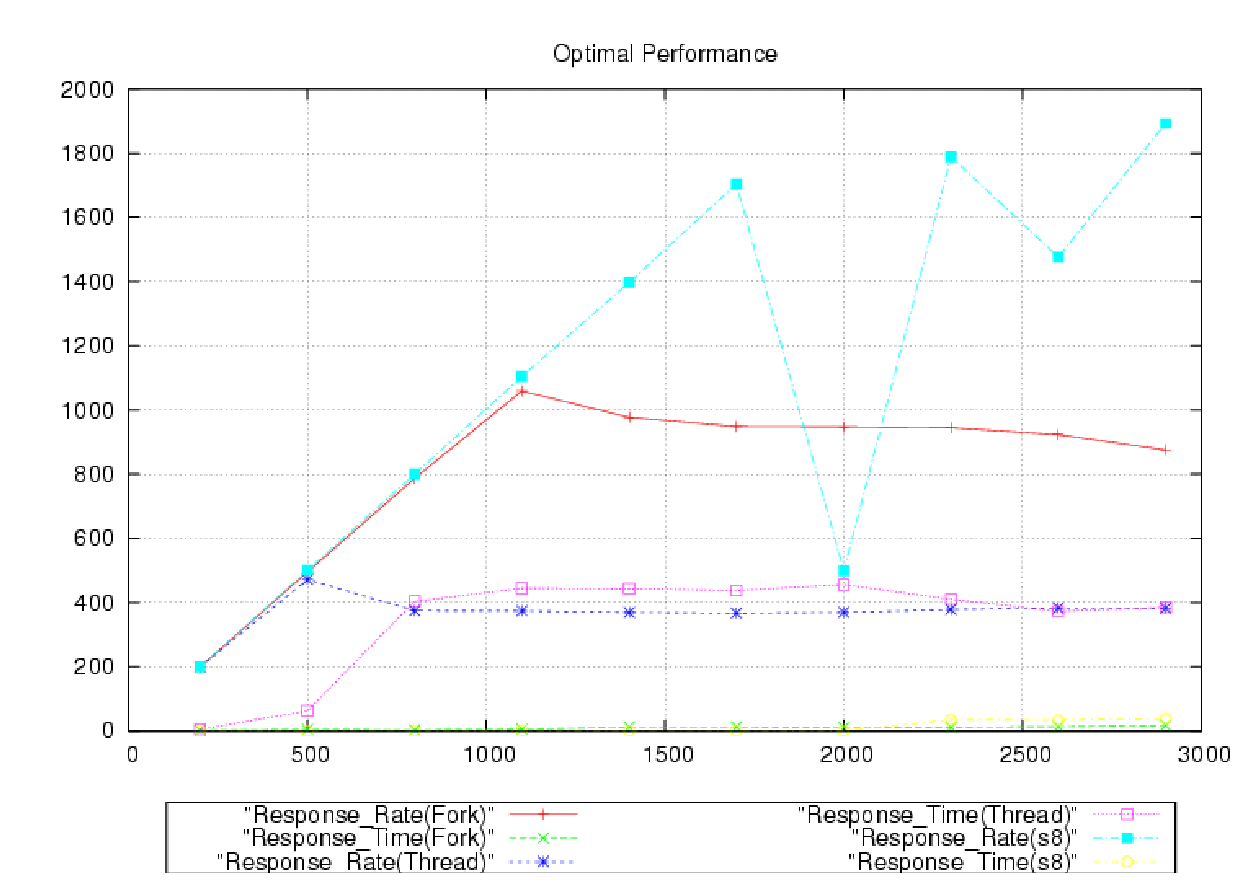
\includegraphics[width=.7\textwidth]{peaks1.eps}
        \caption{Optimal Performance}\label{perfpeak1}
\end{figure}
\begin{figure}[hb]\centering
        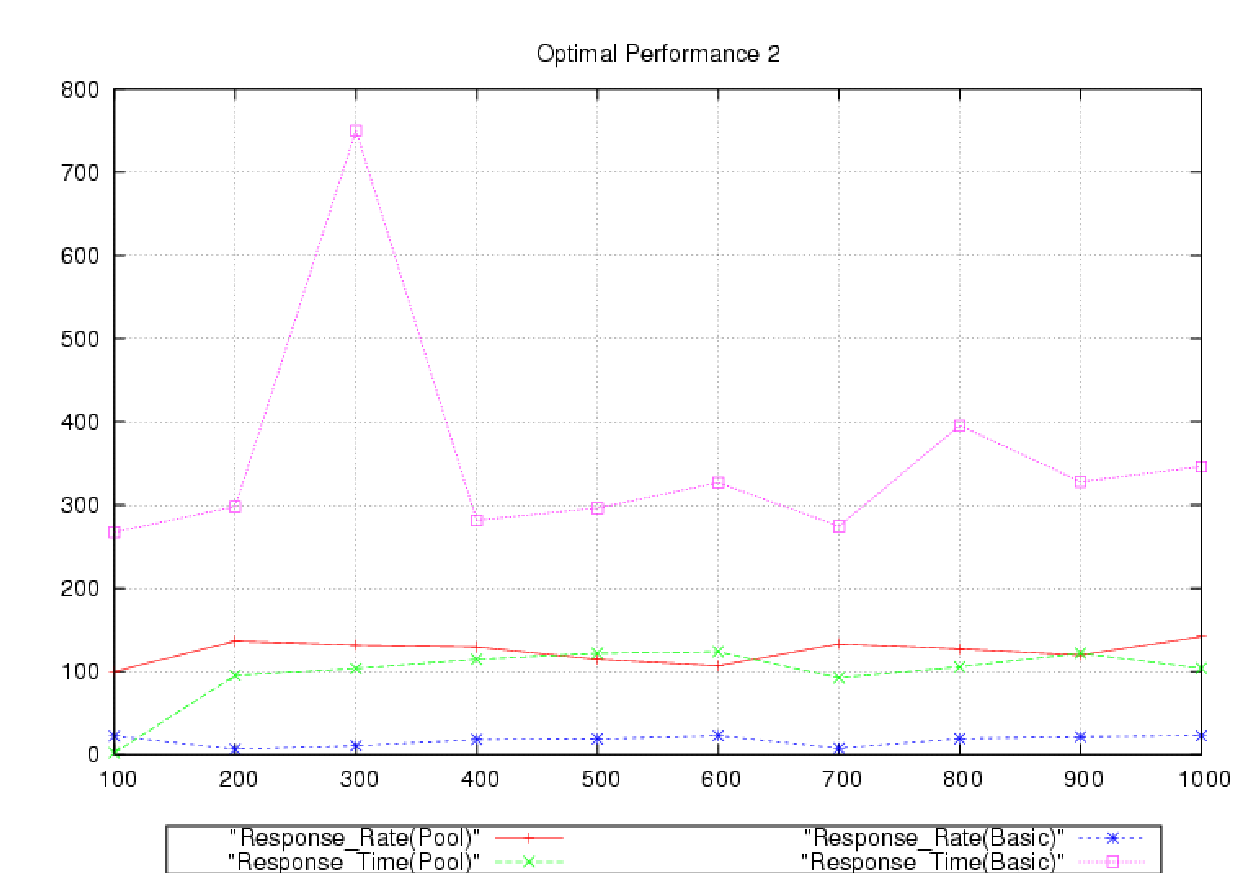
\includegraphics[width=.7\textwidth]{peaks2.eps}
        \caption{Optimal Performance 2}\label{perfpeak2}
\end{figure}

\section{Known Bugs and Errata}\label{bugs}
\subsection{HTTP/1.1 Compliance}
In order to achieve persistent connections, EWE advertises itself as an HTTP/1.1 server.
However, EWE is not in compliance with the HTTP/1.1 standard as given in RFC 2616.
In particular, EWE violates the following `MUST's (see RFC 2119):
\begin{description}
\item[Chunked Data] HTTP/1.1 servers are required to accept requests with chunked data, as outlined in RFC 2616 Section 3.6.
There is no support in EWE for this requirement, so large POST requests will have undefined effects on the server if they are chunk-encoded by the client.
\item[100 Continue response] EWE does not generate the 100 Continue header in response to the client's expectation of such a header.
Because clients that expect this response typically do not rely on it, this oversight is not particularly severe.
However, this header is most often seen in conjunction with large POST requests, and if they are chunk-encoded the request will likely fail anyway.
\item[If-Modified-Since and If-Unmodified-Since] Although EWE sends the Last-Modified header when it is responding with a normal file, it does not process the If-Modified-Since and If-Unmodified-Since conditional requests.
This bug leads to inefficiency for clients that are refreshing their caches.
\end{description}

\subsection{Forked process cleanup}
EWE implements a novel forking system which does not utilize signal calls in zombie cleanup.
This system was necessary because Python does not support blocking signals - only handling or ignoring them.
The cleanup system in EWE will reap all children when certain other events occur, including program exit and receiving a new request.
Because these events may happen infrequently, however, it is possible that several un-reaped zombie children will remain waiting for cleanup until the event occurs.

\subsection{Thread cleanup}
Python does not support killing threads.
Thread removal is often accomplished in Python by having the threads voluntarily exiting when they detect a particular event.
In EWE, this event will never be detected while a thread is handling a client request.
This, when the main program exits, it may inform the user that several threads are still running.
These threads will exit when they are done handling the current request, which may be an indeterminate period of time if a user continues utilizing a persistent connection.

\end{document}
